\documentclass{report}

\usepackage[english]{babel}
\usepackage[letterpaper,top=2cm,bottom=2cm,left=3cm,right=3cm,marginparwidth=1.75cm]{geometry}
\usepackage{amsmath}
\usepackage{graphicx}
\usepackage[colorlinks=true, allcolors=blue]{hyperref}
\graphicspath{{images/}}
\setcounter{tocdepth}{4}
\setcounter{secnumdepth}{4}


\title{Arbitrage Betting}

\author{Mr Ashlin Darius Govindasamy\\ \large{University of South Africa}}

\date{\today}

 

\begin{document}
\maketitle
\newpage
\begin{abstract}
    This paper produces methodologies and ideas on how to do Arbitrage Betting. Arbitrage Betting is explained from first principles mathematically. Source Code for calculating arbitrage bets is also provided in Python. Pros and Cons of Arbitrage Betting are also discussed. Optimization of Arbitrage Betting is also discussed. Real World problems are solved in this paper.
\end{abstract}

\tableofcontents

%for adding page numbers
\pagenumbering{arabic} 


%add more chapters like this
\chapter{Introduction}
\section{Introduction to Arbitrage Betting}
Betting arbitrage ("sure bets", sports arbitrage) is an example of arbitrage arising on betting markets due to either bookmakers' differing opinions on event outcomes or errors. When conditions allow, by placing one bet per each outcome with different betting companies, the bettor can make a profit regardless of the outcome. Mathematically, arbitrage occurs when there are a set of odds, which represent all mutually exclusive outcomes that cover all state space possibilities (i.e. all outcomes) of an event, whose implied probabilities add up to less than 1. In the bettors' slang an arbitrage is often referred to as an arb; people who take advantage of these arbitrage opportunities are called arbers.

\subsection{Theory of Arbitrage Betting}

Consider the variables for a soccer betting market as follows:
Let us suggest that there are there events in a soccer match. \\

\begin{math}
\begin{array}{l}
\text{P}(\text{Home Team Wins}) = p_{1} \\
\text{P}(\text{Draw}) = p_{2} \\
\text{P}(\text{Away Team Wins}) = p_{3} \\
\\
\end{array}
\end{math}

When betting a match a \textit{bookmaker} will offer odds for each of the three possible outcomes. \\

Some examples of odds are as follows: \\

\begin{math}
\begin{array}{l}
\text{Odds}(\text{Home Team Wins}) = o_{1} \\
\text{Odds}(\text{Draw}) = o_{2} \\
\text{Odds}(\text{Away Team Wins}) = o_{3} \\
\\
\end{array}
\end{math}

The purpose of Arbitrage Betting is to find a set of odds that will allow us to make a profit regardless of the outcome of the match. \\

Before we can do this we need to understand the relationship between odds and probabilities. I will explain below how betting odds work. \\

\subsubsection{Learning to Bet}

\textbf{Bet Amount/Punt Amount} When betting on a match you will be asked to place a bet amount. \\
\textbf{Odds} are the ratio of the amount of money that you will win to the amount of money that you bet. \\
\textbf{Probability} is the likelihood of an event occurring. \\
\textbf{Profit} is the amount of money that you will win. \\
\textbf{Return} is the amount of money that you will win plus the amount of money that you bet. \\

\textbf{Example: There is a soccer match between Manchester United vs Everton.} \\

The odds for Manchester United to win are 1.5. \\
The odds for a draw are 3.5. \\
The odds for Everton to win are 5. \\

Now the ratio of the amount of money that you will win to the amount of money that you bet is as follows: \\

\textbf{Manchester United to win} = 1.5 \\
\textbf{Draw} = 3.5 \\
\textbf{Everton to win} = 5 \\

You may be wondering how the odds are calculated. \\

The bookmaker will calculate the odds based on the probability of the event occurring. 
For interest sake Manchester United compared to Everton, Manchester United is the favourite to win. Everton is the underdog. 
The bookmaker will calculate the odds based on the probability of the event occurring. 
The bookmaker will calculate the probability of the event occurring by looking at the history of the teams. There are many factors that the bookmaker will take into account. 
Different bookmakers will have different odds for the same match. This is where we will take advantage later in our paper to do Arbitrage Betting. \\

Lets take a bet for Manchester United to win. \\

\textbf{Bet Amount} = R100 \\
\textbf{P(Manchester United to win)} = 1.5 \\

Our profit is calculated as follows: \\

\begin{math}
\begin{array}{l}
\text{Profit} = (\text{Bet Amount} \times \text{P(Manchester United to win)}) - \text{Bet Amount} \\
\text{Profit} = (R100 \times 1.5) - R100 \\
\text{Profit} = R50 \\
\\
\end{array}
\end{math}

\begin{math}
\begin{array}{l}
\text{Return} = \text{Bet Amount} + \text{Profit} \\
\text{Return} = R100 + R50 \\
\text{Return} = R150 \\
\\
\end{array}
\end{math}

As you can see we have made a profit of R50. \\
If we bet R100 on Manchester United to win we will win R150. \\

But what happens if Everton wins? \\
We will have a loss of R100. \\

Even a draw will result in a loss of R100. \\

This is why we need to find a set of odds that will allow us to make a profit regardless of the outcome of the match. This is when we will use Arbitrage Betting. \\

\subsubsection{Betting on all the Outcomes}

As we have seen above, we can make a profit by betting on Manchester United to win. \\

Let us see what happens if we bet on all the outcomes. \\
We will bet R100 on Manchester United to win, R100 on a draw and R100 on Everton to win in total our investment is R300. \\

Case 1: Manchester United wins. \\

\begin{math}
\begin{array}{l}
\text{Winning} = \text{Bet Amount} \times \text{P(Manchester United to win)} \\
\text{Winning} = R100 \times 1.5 \\
\text{Winning} = R150 \\

\text{Return} = \text{Bet Amount} + \text{Winning} \\
\text{Return} = R100 + R150 \\
\text{Return} = R250 \\

\text{Profit/Loss} = \text{Return} - \text{TotalInvestment} \\
\text{Profit/Loss} = R250 - R300 \\
\text{Loss} = -R50 \\
\\
\end{array}
\end{math}

Case 2: Draw. \\

\begin{math}
\begin{array}{l}
\text{Winning} = \text{Bet Amount} \times \text{P(Draw)} \\
\text{Winning} = R100 \times 3.5 \\
\text{Winning} = R350 \\
\\
\text{Return} = \text{Bet Amount} + \text{Winning} \\
\text{Return} = R100 + R350 \\
\text{Return} = R450 \\
\\
\text{Profit/Loss} = \text{Return} - \text{TotalInvestment} \\
\text{Profit/Loss} = R450 - R300 \\
\text{Profit} = R150 \\
\\
\end{array}
\end{math}

Case 3: Everton wins. \\

\begin{math}
\begin{array}{l}
\text{Winning} = \text{Bet Amount} \times \text{P(Everton to win)} \\
\text{Winning} = R100 \times 5 \\
\text{Winning} = R500 \\
\\
\text{Return} = \text{Bet Amount} + \text{Winning} \\
\text{Return} = R100 + R500 \\
\text{Return} = R600 \\
\\
\text{Profit/Loss} = \text{Return} - \text{TotalInvestment} \\
\text{Profit/Loss} = R600 - R300 \\
\text{Profit} = R300 \\
\\
\end{array}
\end{math}

As we can see by doing this there is times where we will make a profit and times where we will make a loss. In reality the odds wont be exactly the same as the ones that we have used in our example. It is more dangerous to bet on all the outcomes because the odds will be different. \\
There is still risk involved in betting on all the outcomes. \\
But now i will introduce you to Arbitrage Betting where we will make guaranteed profits. \\

\subsubsection{Mathematics of Arbitrage Betting}

\textbf{Arbitrage Betting} is a betting strategy that allows us to make a profit regardless of the outcome of the match. \\

In order to do Arbitrage Betting we need to find a set of odds that will allow us to make a profit regardless of the outcome of the match. \\

\textbf{Assumption:} \\

Let us generate 3 superficial game odds with 3 outcomes that can occur in a game. \\

The odds are as follows: \\

\begin{tabular}{|c|c|c|c|}
\hline
\textit{$M_{n}$} & \textit{$O_1$} & \textit{$O_2$} & \textit{$O_3$} \\
\hline
\text{$M_{1}$} & 1.5 & 3.5 & 5 \\
\hline
\text{$M_{2}$} & 2 & 3.6 & 5 \\
\hline
\text{$M_{3}$} & 1.6 & 12 & 0.5 \\
\hline
\end{tabular} \\

Where $M_{n}$ is the match number, $O_1$ is the odds of the first outcome, $O_2$ is the odds of the second outcome and $O_3$ is the odds of the third outcome. \\



 



    









\chapter{Betting in the Real World}

\section{Finding the most Optimized Arbitrage Bet}

We have learnt how to find arbitrage bets in the previous section. Now we will learn how to find the most optimized arbitrage bet. This is done by finding the most optimized arbitrage bet in the following way:

We look at $n$ amount of bookmakers $B_{}$. We formulate a matrix of $O_{n}$ odds for the same match $M_{n}$\\

I wrote the odds in a form $O{oddtype,matrixentrynumber}$ in the matrix\\

\begin{equation}
    M_{n} = \begin{bmatrix}
        B_{1} & B_{2} & B_{3} & \dots & B_{n} \\
        O_{1,1} & O_{2,3} & O_{3,5} & \dots & O_{4,7} \\
        O_{1,2} & O_{2,4} & O_{3,6} & \dots & O_{4,8} \\
        \vdots & \vdots & \vdots & \ddots & \vdots \\
        O_{1,k} & O_{2,k+1} & O_{3,k+2} & \dots & O_{4,k+3} \\
    \end{bmatrix}
\end{equation}

We then find the most optimized arbitrage bet by finding the maximum value for each row in the matrix $M_{n}$

Resulting in a matrix of $O_{n}$ odds for the same match $M_{n}$

\begin{equation}
    Opt_{M_{n}} = \begin{bmatrix}
        B_{x} & B_{y} & B_{z} & \dots & B_{p} \\
        O_{1,maxentry} & O_{2,maxentry} & O_{3,maxentry} & \dots & O_{n,maxentry} \\
    \end{bmatrix}
\end{equation}

Where $B_{var}$ is the bookmaker with the highest odds for the match $M_{n}$

In theory the more bookmakers we have the more optimized our arbitrage bet will be. The more optimized bet results in yielding a higher profit for the arbitrage bet.\\

But always remember for it to be an arbitrage bet the $A_{n}$ must be less than $1$.

\newpage
\section{Python Class to Compute Arbitrage Bets}

Using the Python Class we can compute arbitrage bets. The Python Class is called Arbitrage. \\
I wrote this class based on the mathmatical logic of arbitrage betting as discussed in the previous sections.\\

The Arbitrage class is defined as follows:

\begin{python}
class Arbitrage:
	def __init__(self,odds,investment):self.odds=odds;self.investment=investment
	def is_arbitrage(self):
		arbitrageP=0
		for odd in self.odds:arbitrageP+=1/odd
		if arbitrageP<1:return True
		else:return False
	def calculate_arbitrage_percentage(self):
		arbitrageP=0
		for odd in self.odds:arbitrageP+=1/odd
		return arbitrageP
	def calculate_arbitrage_roi(self):return self.calculate_arbitrage_stats()['returnOnInvestment']
	def calculate_arbitrage_stats(self):
		arbitrageP=self.calculate_arbitrage_percentage();bArbitrage=self.is_arbitrage();actualProfit=self.investment/arbitrageP-self.investment;IndividualBets=[];returnOnInvestment=actualProfit/self.investment*100;returnOnInvestment=str(returnOnInvestment)+'%';Payouts=[]
		for odd in odds:IndividualBets.append(self.investment*(1/odd/arbitrageP));Payouts.append(self.investment*(1/odd/arbitrageP)*odd)
		return{'arbitrageP':arbitrageP,'bArbitrage':bArbitrage,'actualProfit':actualProfit,'IndividualBets':IndividualBets,'returnOnInvestment':returnOnInvestment,'Payouts':Payouts}
\end{python}

Let us do an example of how to use the Arbitrage class.\\

Assumption: We have computed the best odds for a match from different bookmakers.\\

We have resulted in a matrix of odds for the same match.\\

\begin{equation}
    M_{1} = 
    \begin{bmatrix}
        B_{1} & B_{2} & B_{3} \\
        O_{1} = 2.6 & O_{2} = 7.8 & O_{3} = 5 \\ 
    \end{bmatrix}    
\end{equation}

Let our investment $I$ be $R100$

\begin{python}
odds=[2.6,7.8,5]
investment=100
objArbitrage = Arbitrage(odds, investments)
print(objArbitrage.calculate_arbitrage_stats())
\end{python}

The output of the above code is as follows: \\

\begin{python}
{'arbitrageP': 0.7128205128205127, 'bArbitrage': True, 'actualProfit': 40.28776978417267, 'IndividualBets': [53.956834532374096, 17.985611510791372, 28.057553956834536], 'returnOnInvestment': '40.28776978417267%', 'Payouts': [140.28776978417267, 140.2877697841727, 140.28776978417267]}
\end{python}

\subsubsection{Opportunities from this}

% render image from images/ folder
\begin{wrapfigure}{r}{0.28\textwidth}
    \centering
    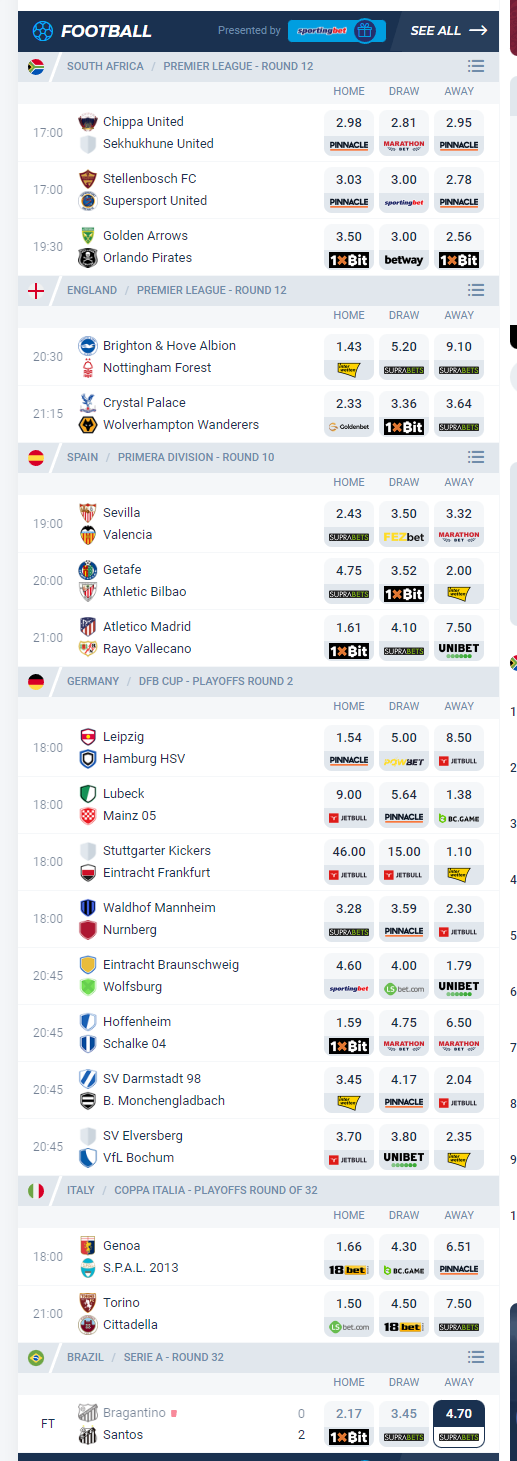
\includegraphics[scale=0.55]{images/oddspedia.png}
    \caption{Oddspedia}
    \label{fig:oddspedia}
\end{wrapfigure}

The above code can be used to compute arbitrage bets.\\

We can use that code to compute arbitrage bets to compute the most optimized arbitrage bet.\\

If we have a matrix of different odds for the same match from different bookmakers. We can compute the most optimized arbitrage bet by finding the maximum value for each row in the matrix $M_{n}$ \\

\begin{math}
    Opt_{n} = \begin{bmatrix}
        B_{x} & B_{y} & B_{z} & \dots & B_{p} \\
        O_{1,maxentry} & O_{2,maxentry} & O_{3,maxentry} & \dots & O_{n,maxentry} \\
    \end{bmatrix}
\end{math} \\

We can introduce Data Science methodologies scrape data from different bookmakers and compute the most optimized arbitrage bet.\\
I wont be showing how to do that in this paper it is up to you to figure that out.\\

There is already websites that do this for you.\\

Example of a website that does this for you: \\ https://oddspedia.com/odds \\

There is also an web application i have developed that does this for you.\\
\\ https://odds.adgstudios.co.za/ \\

It is powered by the Oddspedia API.\\

% center image
\begin{figure}[h]
    \centering
    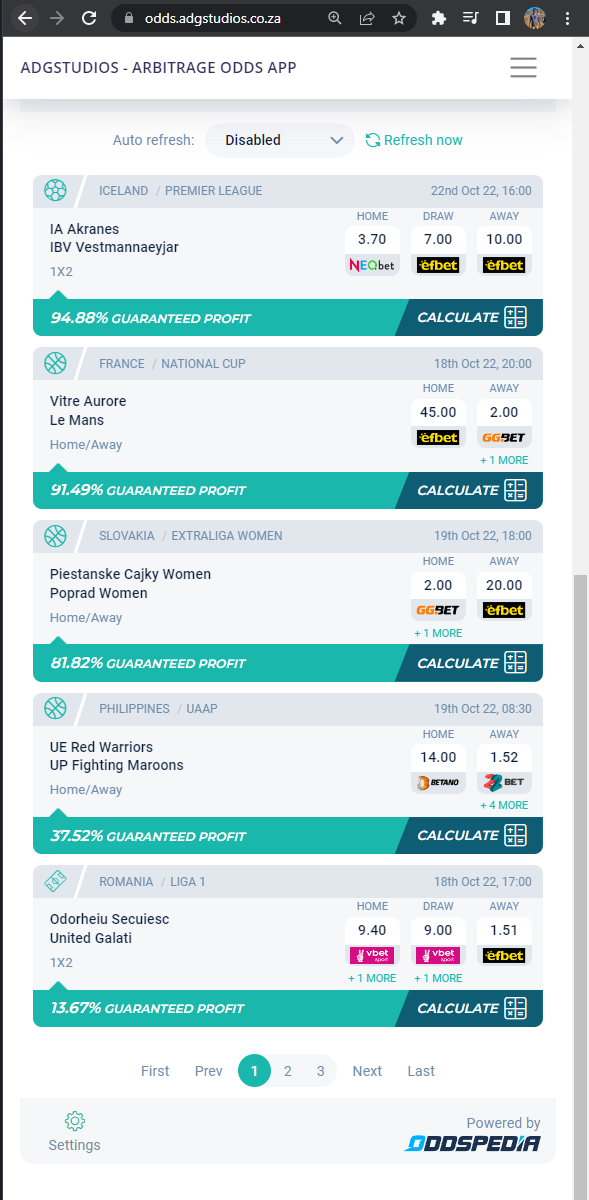
\includegraphics[scale=0.55]{images/arbitrageapp.png}
    \caption{https://odds.adgstudios.co.za/}
    \label{fig:odds}
\end{figure}

\textbf{Limitations of this method:} \\
The websites are not always up to date.\\
Odds change all the time.\\
There are some bookmakers that are not on the websites.\\
Some bookmakers change the odds live during the match.\\
You will have to manually check the odds on the bookmakers website before placing the bet.\\
You will have to have many bookmakers accounts to place the arbitrage bet.\\
Money withdrawal from bookmakers can take a long time.\\







\newpage

\end{document}
